\documentclass[CJK]{beamer}
\usepackage{CJKutf8}
\usepackage{beamerthemesplit}
\usetheme{Malmoe}
\useoutertheme[footline=authortitle]{miniframes}
\usepackage{amsmath}
\usepackage{amssymb}
\usepackage{graphicx}
\usepackage{color}
\usepackage{slashed}
\usepackage{simplewick}
\graphicspath{{../figures/}}
\def\be{\begin{equation}}
\def\ee{\nonumber\end{equation}}
\def\bea{\begin{eqnarray}}
\def\eea{\nonumber\end{eqnarray}}
\def\ii{{\dot{\imath}}}
\def\bch{\begin{CJK}{UTF8}{gbsn}}
\def\ech{\end{CJK}}
\def\bex{\begin{minipage}{0.3\textwidth}
\includegraphics[width=1in]{jugelizi.png}\end{minipage}\begin{minipage}{0.6\textwidth}}
\def\eex{\end{minipage}}
\def\chtitle#1{\frametitle{\bch#1\ech}}
\def\skipline{{\vskip0.1in}}
\def\skiplines{{\vskip0.2in}}
\def\lagr{{\mathcal{L}}}
\def\hamil{{\mathcal{H}}}
\def\vecv{{\mathbf{v}}}
\def\vecx{{\mathbf{x}}}
\def\veck{{\mathbf{k}}}
\def\vecp{{\mathbf{p}}}
\def\vecn{{\mathbf{n}}}
\def\vecA{{\mathbf{A}}}
\def\vecP{{\mathbf{P}}}
\def\vecsigma{{\mathbf{\sigma}}}
\def\hatJn{{\hat{J_\vecn}}}
\def\hatJx{{\hat{J_x}}}
\def\hatJy{{\hat{J_y}}}
\def\hatJz{{\hat{J_z}}}
\def\hatj#1{\hat{J_{#1}}}
\def\hatphi{{\hat{\phi}}}
\def\hatq{{\hat{q}}}
\def\hatpi{{\hat{\pi}}}
\def\vel{\upsilon}
\def\Dint{{\mathcal{D}}}
\def\adag{{\hat{a}^\dagger}}
\def\bdag{{\hat{b}^\dagger}}
\def\cdag{{\hat{c}^\dagger}}
\def\ddag{{\hat{d}^\dagger}}
\def\hata{{\hat{a}}}
\def\hatb{{\hat{b}}}
\def\hatc{{\hat{c}}}
\def\hatd{{\hat{d}}}
\def\hatN{{\hat{N}}}
\def\hatH{{\hat{H}}}
\def\hatp{{\hat{p}}}
\def\Fup{{F^{\mu\nu}}}
\def\Fdown{{F_{\mu\nu}}}
\def\newl{\nonumber \\}
\def\SIkm{\mathrm{km}}
\def\SIyr{\mathrm{yr}}
\def\SIGyr{\mathrm{Gyr}}
\def\SIeV{\mathrm{eV}}
\def\SIGeV{\mathrm{GeV}}
\def\SIm{\mathrm{m}}
\def\SIcm{\mathrm{cm}}
\def\SIJ{\mathrm{J}}
\def\SIs{\mathrm{s}}
\def\SIkg{\mathrm{kg}}
\def\SIg{\mathrm{g}}
\def\vece{\mathrm{e}}
\def\bmat#1{\left(\begin{array}{#1}}
\def\emat{\end{array}\right)}
\def\bcase#1{\left\{\begin{array}{#1}}
\def\ecase{\end{array}\right.}
\def\calM{{\mathcal{M}}}
\def\calT{{\mathcal{T}}}
\def\calR{{\mathcal{R}}}
\def\barpsi{\bar{\psi}}
\def\baru{\bar{u}}
\def\barv{\bar{\upsilon}}
\def\bmini#1{\begin{minipage}{#1\textwidth}}
\def\emini{\end{minipage}}
\def\qeq{\stackrel{?}{=}}
\def\torder#1{\mathcal{T}\left(#1\right)}
\def\rorder#1{\mathcal{R}\left(#1\right)}


\title{Quantum Field Theory I \\ Lesson 18 - Openmind I}
\author{}
\date{}


\begin{document}

\begin{frame}
 
\begin{center}
\begin{Large}
\bch
量子场论 I 

{\vskip 0.3in}

第十八课 脑洞大开系列(一)

\ech
\end{Large}
\end{center}

\vskip 0.2in

\bch
课件下载
\ech
https://github.com/zqhuang/SYSU\_QFTI

\end{frame}


\begin{frame}
\chtitle{解决物理问题的正确方法}
\bch
解决物理问题的正确方法:
\begin{itemize}
\item[1]{理解问题中的物理量的量纲和含义}
\item[2]{用对称性分析,量纲分析,简单的物理原则,或者取某些特殊情况估算答案的形式或数量级}
\item[3]{写下系统的运动方程并求解}
\item[4]{将答案和第2步做比较}
\end{itemize}

\skipline
步骤1,2,4往往被跳过,那是因为你解的题目有意被设计成书上例题的翻版。总是这样学习的话,遇到不熟悉的问题只会束手无策。

\ech
\end{frame}


\begin{frame}
\chtitle{例子1}
\bch
试估算地球表面的大气分子之间的势能大小。
\ech
\end{frame}


\begin{frame}
\chtitle{例子2}
\bch
一个半径约为$100$光年的球状星团中恒星的典型速度约为$100\SIkm/\SIs$。假设恒星的典型质量为太阳质量($\sim 10^{30}\SIkg$)。估算该球状星团中大约有多少颗恒星。
\ech
\end{frame}



\begin{frame}
\chtitle{例子3}
\bch
一维无限深势阱的宽度为$L$,试计算势阱中质量为$m$的粒子的基态能量。
\ech
\end{frame}



\begin{frame}
\chtitle{例子4}
\bch
黑洞可以看成一个把物质束缚在视界内的“势阱”
\begin{itemize}
\item{中性不旋转的黑洞的视界是什么形状}
\item{估算质量为$M$的中性不旋转的黑洞的视界大小}
\item{Hawking通过把量子理论在平直时空外推的方法计算出黑洞有辐射且有温度,试估算估算质量为$M$的中性不旋转的黑洞的温度(假设观测者在远处)}
\end{itemize}
\ech
\end{frame}

\begin{frame}
\chtitle{课堂讨论:例子5}
\bch
相对论里能量动量张量$T^{\mu\nu}$是对牛顿力学里的质量密度的推广。对静止的理想流体$T^{\mu\nu} = \mathrm{diag}(\rho, p, p, p)$,其中$\rho$是流体的能量密度,$p$是流体的压强。

牛顿引力理论里的质量密度就被推广为能量动量张量的迹$\mathrm{Tr}(T^{\mu\nu}) = \rho + 3p$。质量为$M$的大质量天体对附近物质的牛顿引力公式可以推广到
$$ F = - \int d^3\vecx \frac{GM(\rho + 3p) \vec{r}}{r^3}$$
光子和质子以相同速度和入射角通过太阳附近,由于受到太阳引力而造成的偏折角分别为$\theta_\gamma$和$\theta_p$,求$\theta_\gamma/\theta_p$。

\ech
\end{frame}

\begin{frame}
\chtitle{理科PhD学生第一守则}
\bch
拿到问题不知道该干嘛时,先做个傅立叶变换。
\ech
\end{frame}

\begin{frame}
\chtitle{养成到“对角化”空间考虑问题的习惯}
\bch

{\small任何拉氏量为二次型的系统都是“自由场”。把拉氏量对角化是透过迷雾看本质的有效方法。

\skipline
 第一守则的由来:当拉氏量里包含了空间偏导时,傅立叶变换往往能成功地把拉氏量对角化。}

\ech
\end{frame}

\begin{frame}
\chtitle{课堂讨论}
\bch
怎样把变量为$x^1, x^2,\ldots, x^n$的拉氏量
$$L = \frac{1}{2} (\dot{x}^i-v^i) K_{ij} (\dot{x}^j-v^j) - \frac{1}{2} (x^i-b^i) V_{ij} (x^j - b^j)$$
通过变量替换的方法变为$n$个独立谐振子的拉氏量之和?
\ech
\end{frame}


\begin{frame}
\chtitle{例子6}
\bch
\bmini{0.6}
如图,无重力的空间中,质量为$m_1$和$m_2$的两个质点固定在弹性系数为$k$,长度为$L$的弹簧两端。如果在$t=0$时刻把弹簧压缩到$L/2$后释放,求两个质点之后的位置随时间的变化。
\emini
\bmini{0.35}
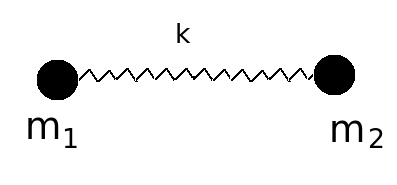
\includegraphics[width=1.8in]{doubleosc.png}
\emini
\ech
\end{frame}


\begin{frame}
\chtitle{例子7}
\bch
\bmini{0.6}
如图,无重力的空间中,质量为$m_1$和$m_2$的两个质点固定在弹性系数为$k$的弹簧两端。求该系统的量子零点能。

\skipline
思考:该结果和弹簧长度或者参考系有关吗?
\emini
\bmini{0.35}
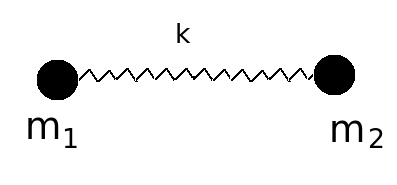
\includegraphics[width=1.8in]{doubleosc.png}
\emini
\ech
\end{frame}

\end{document}


